\subsection{Other Movement}
To keep movement somewhat varied and not have characters either require path finding or be idle, we thought of some other movements to keep characters busy in a relatively cheap way. Just as path following, these alternate movements should make use of steering behaviour and follow the same repulsion rules for other characters and obstacles. The two primary alternate movements we went for are leader following and wandering.

\subsubsection{Leader Following}
Characters in real-time strategy games often benefit from travelling in groups. Zombies have a form of group behaviour, while vikings can be commanded in groups. When moving groups, it is usually convenient to define a leader and simply have the rest move along with the leader.

Our desired way of leader following relies on steering behaviour, but we did not get far enough in development to implement this. In order to follow the leader, all followers will use seeking behaviour on a point slightly behind the leader. Next to this, the followers should not be in the way of the leader, so they use fleeing behaviour on a point slightly in front of the leader. Both of these behaviours are described in section \ref{sec:pathfollowing}.

Instead, we simply let the leader of a group apply path finding. The followers simply get the path assigned by the leader and all follow the path independently. This keeps performance decent by only requiring the leader to run path finding. A property of this approach is that the leader is not necessarily in front. The main problem with this approach is that the nature of our path following makes the group somewhat converge into a line over time. This is caused by the frequent updates in target and the close proximity these target have to the location of the characters.

\subsubsection{Wandering}
Zombies will want to explore the map and search for vikings or other things on the map they can influence to their advantage. When not knowing much about the map around you, wandering is the best thing you can do to search, outside of applying intelligent searching techniques. 
\begin{wrapfigure}{r}{0.30\textwidth}
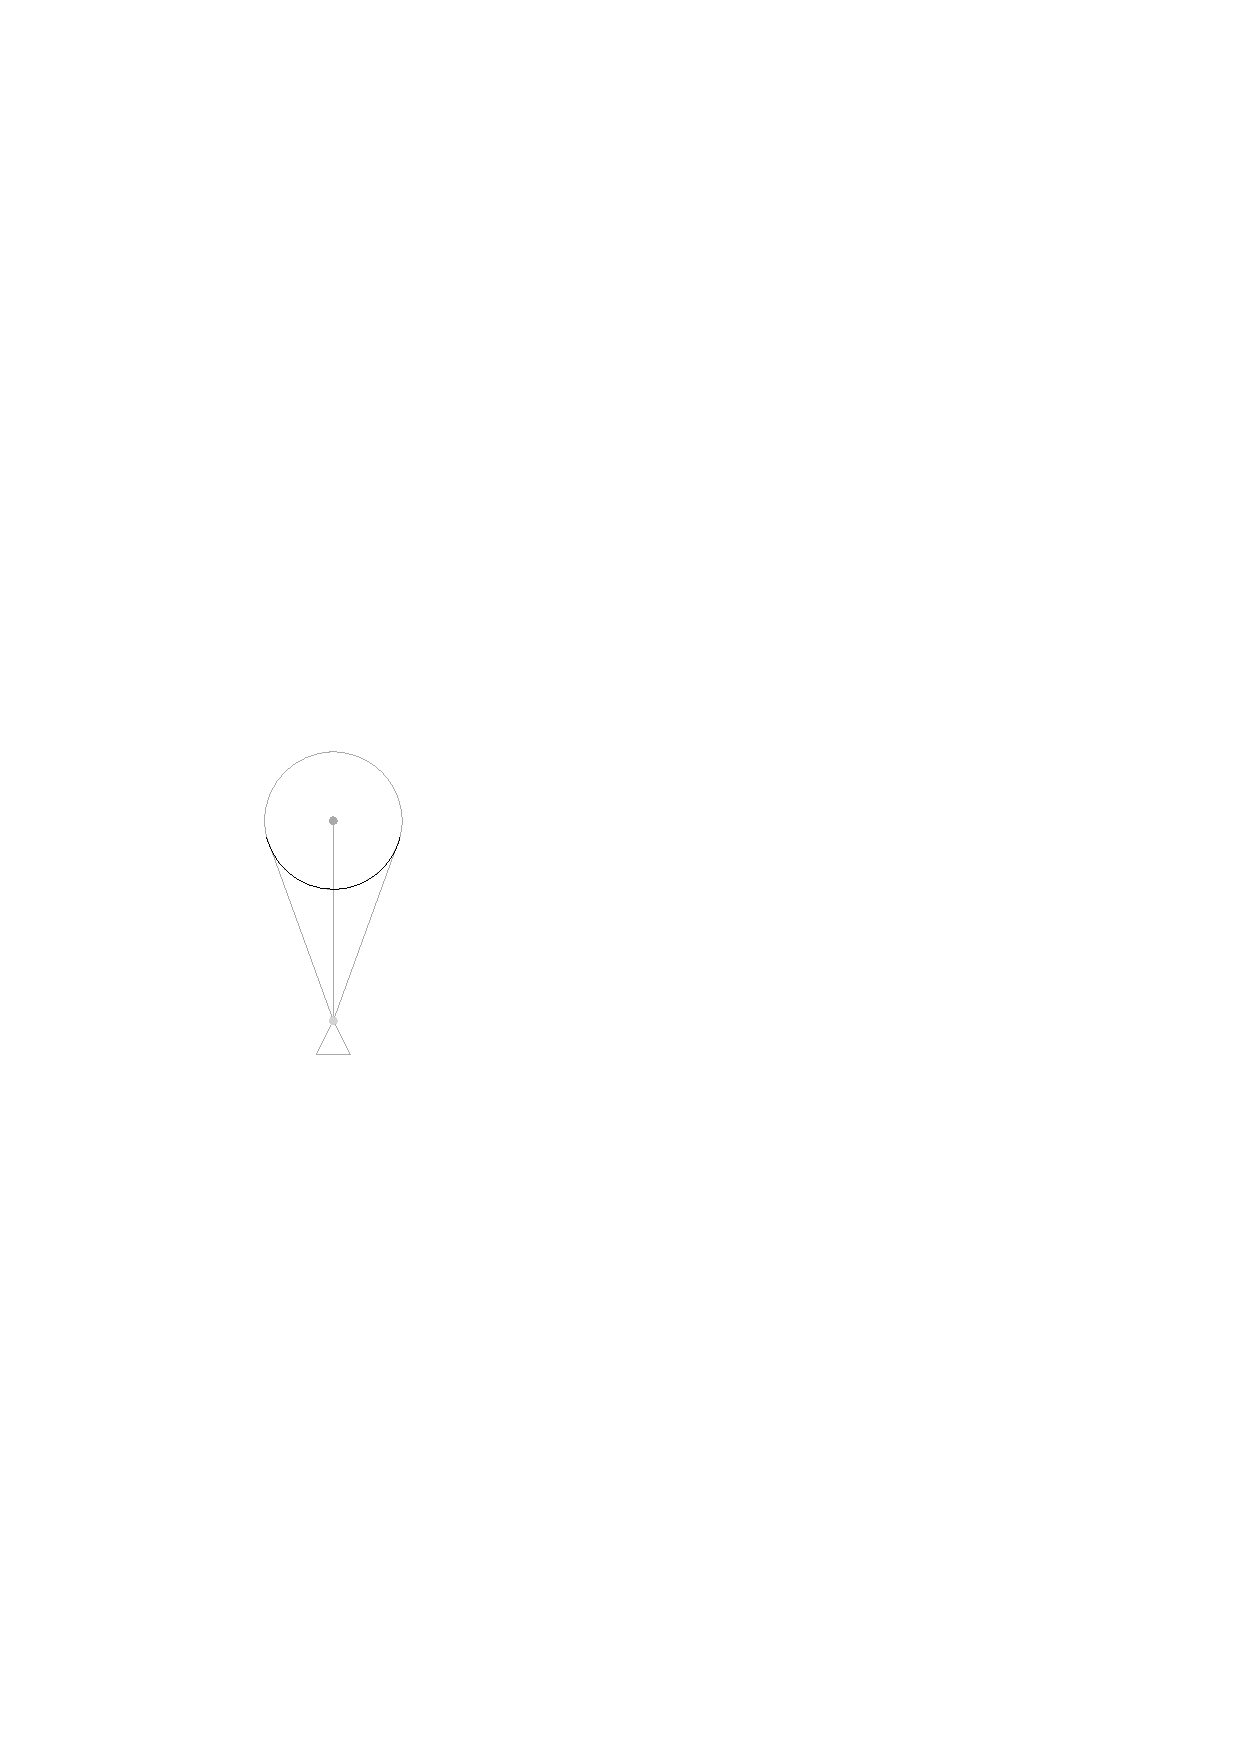
\includegraphics[width=0.30\textwidth]{../images/useless_angle.pdf}
\caption{Useless angles}
\label{fig:tangents}
\end{wrapfigure}

Our desired way of wandering also relies on steering behaviour, sadly we did not have time to implement this into the game. Proper wandering behaviour is done essentially by considering a circle some distance in front of the wandering character and taking a random angle on that circle as the vector to be added to the current direction. More specifically, the force is the sum of the vector from the character to the center of the circle, and the vector from the center of the circle to the edge of it. The farther the circle is away from the character, the more force is calculated in from the current direction. The larger the circle is, the more force from the random angle is calculated into the new direction. The degree to which the direction on the circle is allowed to deviate from straight also in part determines how sharp the turns are the character can take. If the end of the vector on the circle lies farther from straight than the intersection between the circle and the tangent lines of the circle through the character (figure \ref{fig:tangents}, marked black), the effect becomes a duplicate of an existing possibility. This is due to the vector being normalized and scaled to a constant speed after the direction is determined.

The way we ended up improvising wandering behaviour is by having zombies use path finding anyway. The path they find is simply one towards a randomly selected point in a small radius around them. A new random path is calculated at regular time intervals, shorter than the time it takes to complete the path, as to keep on the move. This wandering approach does not render realistic or efficient wandering behaviour, but it was all we could get in given the time constraints and priority.
